% alfak2 sparse joint model: how fit_sparse_joint() chooses its path.
% Mirrors fit_sparse_joint() in R/sparse-joint.R and the series methods in
% R/sparse-joint-series-methods.R. Build: pdflatex flow_overview.tex
\documentclass[tikz,border=4pt]{standalone}
% Shared style of the alfak2 flowcharts (doc/flowcharts/*.tex).
% Each chart is a standalone document; build one with
%   cd doc/flowcharts && pdflatex <chart>.tex
% or all of them with doc/flowcharts/build.sh. doc/alfak2_method.tex includes
% the PDFs.
\usepackage{amsmath,amssymb}
\usepackage[scaled=0.92]{helvet}
\renewcommand{\familydefault}{\sfdefault}
\usepackage{xcolor}
\usetikzlibrary{positioning,shapes.geometric,shapes.misc,arrows.meta,calc,fit,backgrounds}

% Thresholds of series = "auto" (sparse_joint_auto_thresholds in
% R/sparse-joint-series-methods.R). Change them here when the code changes.
\newcommand{\autoshare}{0.3}
\newcommand{\autoweight}{0.5}

\newcommand{\code}[1]{\texttt{\small #1}}

\definecolor{cIn}{HTML}{DCE6F2}    \definecolor{cInB}{HTML}{4F6D9A}
\definecolor{cProc}{HTML}{F5F5F5}  \definecolor{cProcB}{HTML}{707070}
\definecolor{cDec}{HTML}{FFF2CC}   \definecolor{cDecB}{HTML}{B8902B}
\definecolor{cTwo}{HTML}{D0E4F5}   \definecolor{cTwoB}{HTML}{2E6DA4}
\definecolor{cAnch}{HTML}{D9EAD3}  \definecolor{cAnchB}{HTML}{3D7A33}
\definecolor{cPair}{HTML}{FCE5CD}  \definecolor{cPairB}{HTML}{C0661A}
\definecolor{cState}{HTML}{E6DDF2} \definecolor{cStateB}{HTML}{6A4A9C}
\definecolor{cCore}{HTML}{EFEFEF}  \definecolor{cCoreB}{HTML}{8A8A8A}
\definecolor{cOut}{HTML}{D5EDEA}   \definecolor{cOutB}{HTML}{2C7C73}
\definecolor{cErr}{HTML}{F8D7D7}   \definecolor{cErrB}{HTML}{B03030}
\definecolor{cAuto}{HTML}{FFFBEA}

\tikzset{
  >={Stealth[length=2.4mm,width=1.8mm]},
  every node/.style={font=\small},
  box/.style={draw=#1B, fill=#1, rounded corners=2.5pt, line width=0.7pt, align=left,
              inner xsep=5pt, inner ysep=4pt},
  box/.default=cProc,
  w/.style={text width=#1},
  dec/.style={draw=cDecB, fill=cDec, chamfered rectangle, chamfered rectangle xsep=7pt,
              line width=0.7pt, align=center, inner xsep=3pt, inner ysep=3pt},
  err/.style={box=cErr, font=\footnotesize},
  tag/.style={draw=#1, dashed, rounded corners=6pt, fill=white, font=\scriptsize, inner sep=2.5pt,
              align=center},
  arr/.style={->, line width=0.8pt, draw=black!75},
  darr/.style={->, line width=0.8pt, draw=black!60, dashed},
  lab/.style={font=\footnotesize\itshape, fill=white, inner sep=1.5pt, text=black!85},
  frame/.style={draw=#1, rounded corners=6pt, line width=0.9pt, inner sep=7pt},
  ftitle/.style={font=\footnotesize\bfseries, fill=white, inner sep=2pt, text=#1},
}

\begin{document}
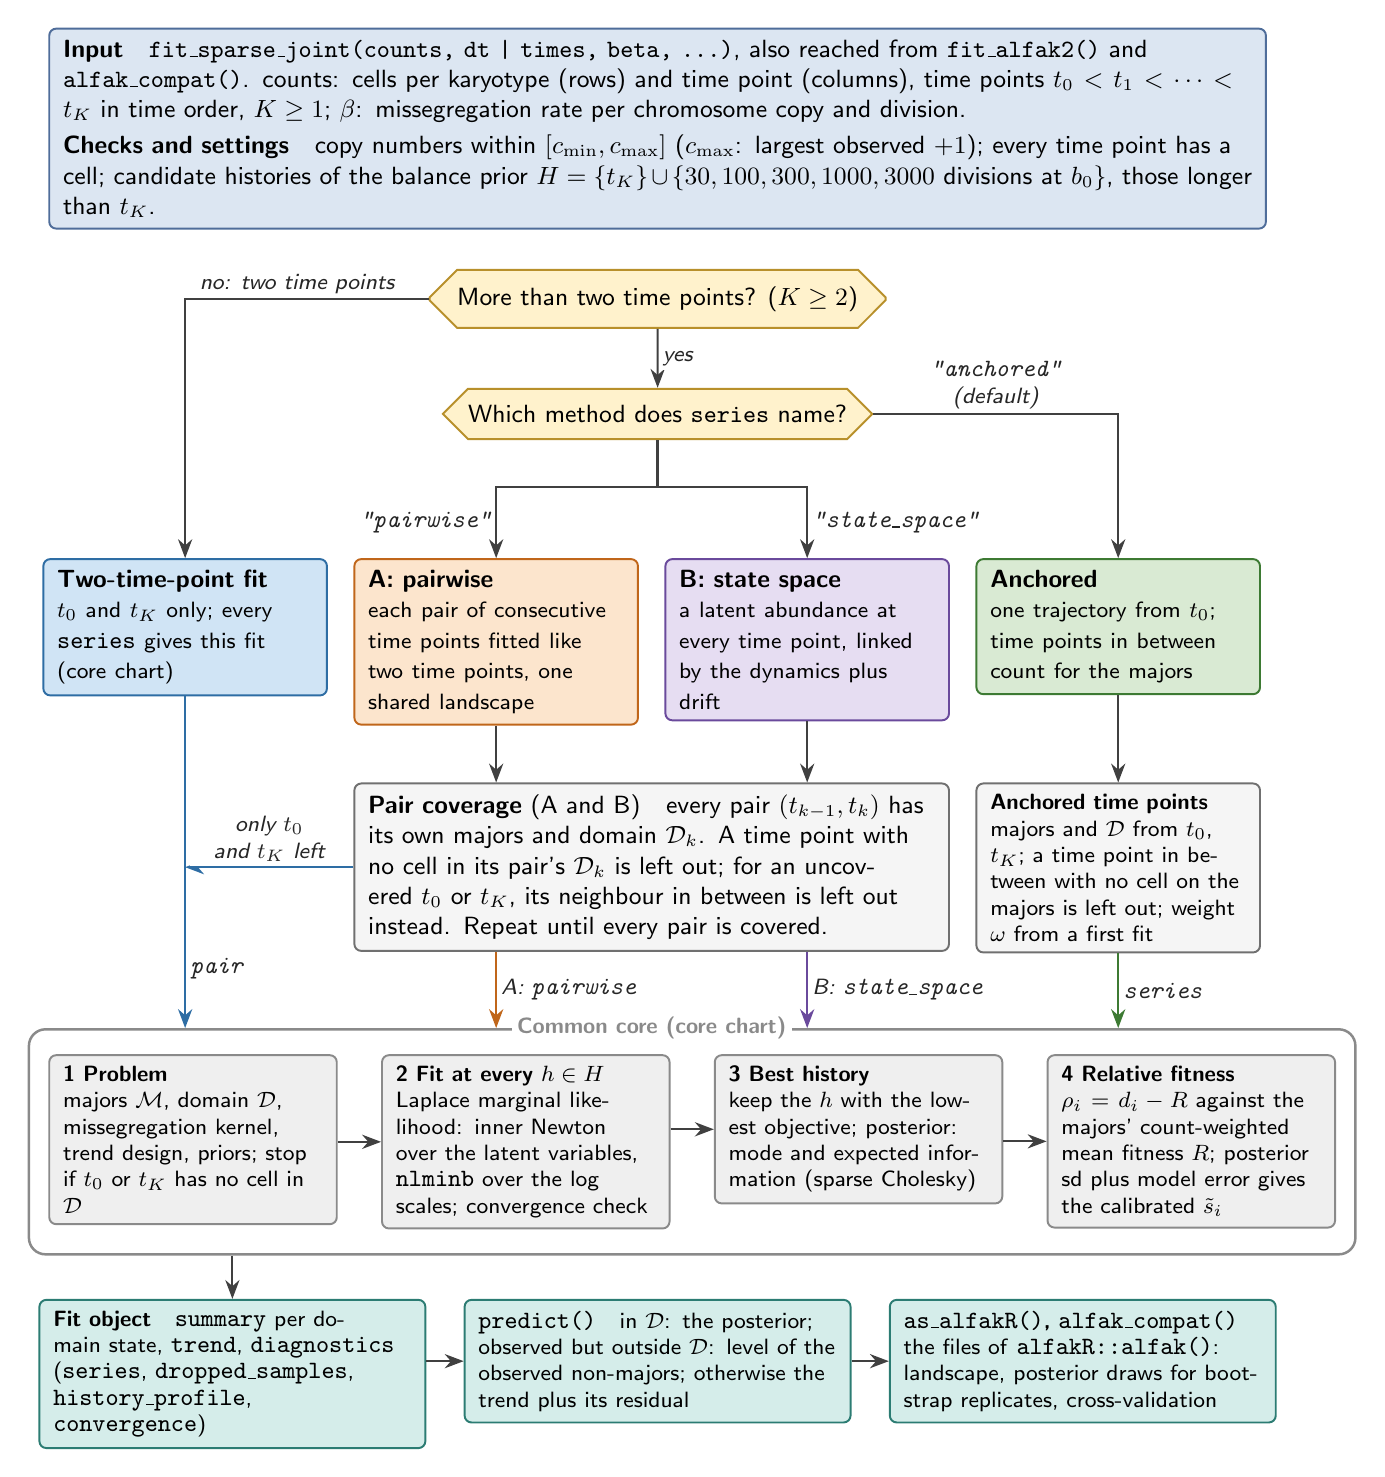
\begin{tikzpicture}

% ---- input and checks ---------------------------------------------------
\node[box=cIn, w=15.1cm] (in) at (7.85,0) {%
  \textbf{Input}\quad \code{fit\_sparse\_joint(counts, dt | times, beta, \ldots)}, also reached from
  \code{fit\_alfak2()} and \code{alfak\_compat()}. counts: cells per karyotype (rows) and time point (columns),
  time points $t_0<t_1<\dots<t_K$ in time order, $K\ge1$; $\beta$: missegregation rate per chromosome copy and
  division.\\[2pt]
  \textbf{Checks and settings}\quad copy numbers within $[c_{\min},c_{\max}]$ ($c_{\max}$: largest observed
  $+1$); every time point has a cell; candidate histories of the balance prior
  $H=\{t_K\}\cup\{30,100,300,1000,3000 \text{ divisions at } b_0\}$, those longer than $t_K$.};
\coordinate (chk) at (in.south);

% ---- number of time points and series -----------------------------------------
\node[dec, below=0.5cm of chk] (many) {More than two time points? ($K\ge2$)};
\node[dec, below=0.75cm of many] (series) {Which method does \code{series} name?};
\draw[arr] (many) -- node[lab, right] {yes} (series);

% ---- the four paths ------------------------------------------------------------
\path (series.south) ++(0,-1.5) coordinate (rowtop);
\node[box=cTwo,   w=3.25cm, anchor=north] (two)  at (1.85,  0 |- rowtop) {%
  \textbf{Two-time-point fit}\\{\footnotesize $t_0$ and $t_K$ only; every \code{series} gives this fit (core chart)}};
\node[box=cPair,  w=3.25cm, anchor=north] (pair) at (5.8,   0 |- rowtop) {%
  \textbf{A: pairwise}\\{\footnotesize each pair of consecutive time points fitted like two time points, one shared landscape}};
\node[box=cState, w=3.25cm, anchor=north] (ss)   at (9.75,  0 |- rowtop) {%
  \textbf{B: state space}\\{\footnotesize a latent abundance at every time point, linked by the dynamics plus drift}};
\node[box=cAnch,  w=3.25cm, anchor=north] (anch) at (13.7,  0 |- rowtop) {%
  \textbf{Anchored}\\{\footnotesize one trajectory from $t_0$; time points in between count for the majors}};

% the user's choice into the paths
\path (series.south) ++(0,-0.6) coordinate (split);
\draw[arr] (series.south) -- (split) -| node[lab, pos=0.75, left] {\code{"pairwise"}} (pair.north);
\draw[arr] (split) -| node[lab, pos=0.75, right] {\code{"state\_space"}} (ss.north);
\draw[arr] (series.east) -| node[lab, pos=0.25, above, align=center] {\code{"anchored"}\\(default)} (anch.north);
\draw[arr] (many.west) -| node[lab, pos=0.27, above] {no: two time points} (two.north);

% ---- leaving time points out ----------------------------------------------------------
\node[box, w=7.2cm, anchor=north] (pc) at ($(pair.south)!0.5!(ss.south)+(0,-0.75)$) {%
  \textbf{Pair coverage} (A and B)\quad every pair $(t_{k-1},t_k)$ has its own majors and domain
  $\mathcal D_k$. A time point with no cell in its pair's $\mathcal D_k$ is left out; for an uncovered
  $t_0$ or $t_K$, its neighbour in between is left out instead. Repeat until every pair is covered.};
\node[box, w=3.25cm, anchor=north, font=\footnotesize] (ac) at (anch.south |- pc.north) {%
  \textbf{Anchored time points}\quad majors and $\mathcal D$ from $t_0$, $t_K$; a time point in between with
  no cell on the majors is left out; weight $\omega$ from a first fit};
\draw[arr] (pair.south) -- (pair.south |- pc.north);
\draw[arr] (ss.south) -- (ss.south |- pc.north);
\draw[arr] (anch) -- (ac);

% ---- common core --------------------------------------------------------------------
\path (pc.south) ++(0,-1.3) coordinate (coretop);
\node[box=cCore, w=3.3cm, anchor=north, font=\footnotesize] (c1) at (1.95, 0 |- coretop) {%
  \textbf{1 Problem}\\ majors $\mathcal M$, domain $\mathcal D$, missegregation kernel, trend design,
  priors; stop if $t_0$ or $t_K$ has no cell in $\mathcal D$};
\node[box=cCore, w=3.3cm, anchor=north west, font=\footnotesize] (c2) at ($(c1.north east)+(0.55,0)$) {%
  \textbf{2 Fit at every $h\in H$}\\ Laplace marginal likelihood: inner Newton over the latent
  variables, \code{nlminb} over the log scales; convergence check};
\node[box=cCore, w=3.3cm, anchor=north west, font=\footnotesize] (c3) at ($(c2.north east)+(0.55,0)$) {%
  \textbf{3 Best history}\\ keep the $h$ with the lowest objective; posterior: mode and expected
  information (sparse Cholesky)};
\node[box=cCore, w=3.3cm, anchor=north west, font=\footnotesize] (c4) at ($(c3.north east)+(0.55,0)$) {%
  \textbf{4 Relative fitness}\\ $\rho_i=d_i-R$ against the majors' count-weighted mean fitness $R$;
  posterior sd plus model error gives the calibrated $\tilde s_i$};
\draw[arr] (c1.east |- c2.west) -- (c2.west);
\draw[arr] (c2.east |- c3.west) -- (c3.west);
\draw[arr] (c3.east |- c4.west) -- (c4.west);
\begin{scope}[on background layer]
  \node[frame=cCoreB, fill=white, fit=(c1)(c2)(c3)(c4), inner ysep=9pt] (core) {};
\end{scope}
\node[ftitle=cCoreB] at ($(pair.south |- core.north)!0.5!(ss.south |- core.north)$) {Common core (core chart)};

% paths into the core, with their TMB template
\draw[arr, draw=cTwoB] (two.south) -- node[lab, pos=0.82, right] {\code{pair}} (two.south |- core.north);
\draw[arr, draw=cPairB] (pair.south |- pc.south) -- node[lab, right] {A: \code{pairwise}} (pair.south |- core.north);
\draw[arr, draw=cStateB] (ss.south |- pc.south) -- node[lab, right] {B: \code{state\_space}} (ss.south |- core.north);
\draw[arr, draw=cAnchB] (ac.south) -- node[lab, right] {\code{series}} (ac.south |- core.north);
% fallback to the two-time-point fit
\draw[arr, draw=cTwoB] (pc.west) -- node[lab, above, align=center, text width=1.9cm] {only $t_0$ and $t_K$ left} (pc.west -| two.south);

% ---- output ----------------------------------------------------------------------------
\path (core.south) ++(0,-0.55) coordinate (outtop);
\node[box=cOut, w=4.55cm, anchor=north, font=\footnotesize] (o1) at (2.45, 0 |- outtop) {%
  \textbf{Fit object}\quad \code{summary} per domain state, \code{trend},
  \code{diagnostics} (\code{series}, \code{dropped\_samples}, \code{history\_profile},
  \code{convergence})};
\node[box=cOut, w=4.55cm, anchor=north, font=\footnotesize] (o2) at (7.85, 0 |- outtop) {%
  \textbf{\code{predict()}}\quad in $\mathcal D$: the posterior; observed but outside $\mathcal D$:
  level of the observed non-majors; otherwise the trend plus its residual};
\node[box=cOut, w=4.55cm, anchor=north, font=\footnotesize] (o3) at (13.25, 0 |- outtop) {%
  \textbf{\code{as\_alfakR()}, \code{alfak\_compat()}}\quad the files of \code{alfakR::alfak()}:
  landscape, posterior draws for bootstrap replicates, cross-validation};
\draw[arr] (core.south -| o1.north) -- (o1.north);
\draw[arr] (o1.east |- o2.west) -- (o2.west);
\draw[arr] (o2.east |- o3.west) -- (o3.west);

\end{tikzpicture}
\end{document}
